\documentclass{article}

\usepackage{graphicx} % Required for including images
\usepackage{booktabs} % For prettier tables
\usepackage{hyperref} % For hyperlinks in the PDF
\usepackage{bookmark} % more advanced and customizable bookmark structure

\usepackage{lmodern}  % for bold teletype font
\usepackage{amsmath}  % for \hookrightarrow
\usepackage{xcolor}
\usepackage{listings}

\lstset{
  basicstyle=\ttfamily,
  columns=fullflexible,
  frame=single,
  breaklines=true,
  postbreak=\mbox{\textcolor{red}{$\hookrightarrow$}\space},
}

\title{Post Office Reservation Database \\ \large Database and Management Project}

\author{Alessandro Vecchi \and Francesco Danese}
\date{\today}

\begin{document}

\maketitle

\begin{abstract}
The report presents a project for the Data Management and Analysis course. The project consists of the design and implementation of a database system for managing reservations at a post office. The database is implemented in PostgreSQL and populated with sample data.
\end{abstract}

\section{Introduction}
% Describe the project here
This database is designed to manage the operations of a Post Office. It keeps track of users, postal workers, services offered, and reservations made for these services.

In the following section we are going to write the detailed description of the database we realized, along with the constraints and the trigger considered. Then we will show the ER diagram and the relational schema of the database. Finally, we will show the SQL code used to create the database and we will populate it with sample data.
\section{Database Design}
% Describe the database design here
The database consists of four main tables: Users, PostalWorker, Service, and Reservation.

The Users table stores information about the users of the post office services. Each user is uniquely identified by their fiscal code, which follows the pattern of the Italian fiscal code. Other information stored about each user includes their name, surname, date of birth, email (which is optional), city, ZIP code (CAP), and address. The ZIP code must be exactly 5 digits long.

The PostalWorker table stores information about the postal workers. Each postal worker is uniquely identified by their ID\@. Other information stored about each postal worker includes their RAL, name, surname, and email. The email must be unique across all postal workers, and the RAL must be greater than 0.

The Service table stores information about the services offered by the post office. Each service is uniquely identified by its type. Other information stored about each service includes the maximum time it takes and its price. The maximum time is stored as a time value, and the price must be greater than 0.

The Reservation table stores information about the reservations made by users for the services. Each reservation is uniquely identified by its reservation ID\@. Other information stored about each reservation includes the date, time, user fiscal code, postal worker ID, and type of service. The user fiscal code, postal worker ID, and type of service are foreign keys referencing the Users, PostalWorker, and Service tables, respectively.

The database also includes a trigger to prevent a user from booking two services that overlap in time. Before a new reservation is inserted or an existing reservation is updated, the trigger checks if the user has any other reservations at the same date and time that overlap with the new or updated reservation. If such an overlapping reservation exists, the trigger raises an exception and prevents the operation from completing.

This database design allows the post office to efficiently manage its operations, ensure the integrity of its data, and enforce its business rules.

This is the ER diagram of the database:
\begin{center}
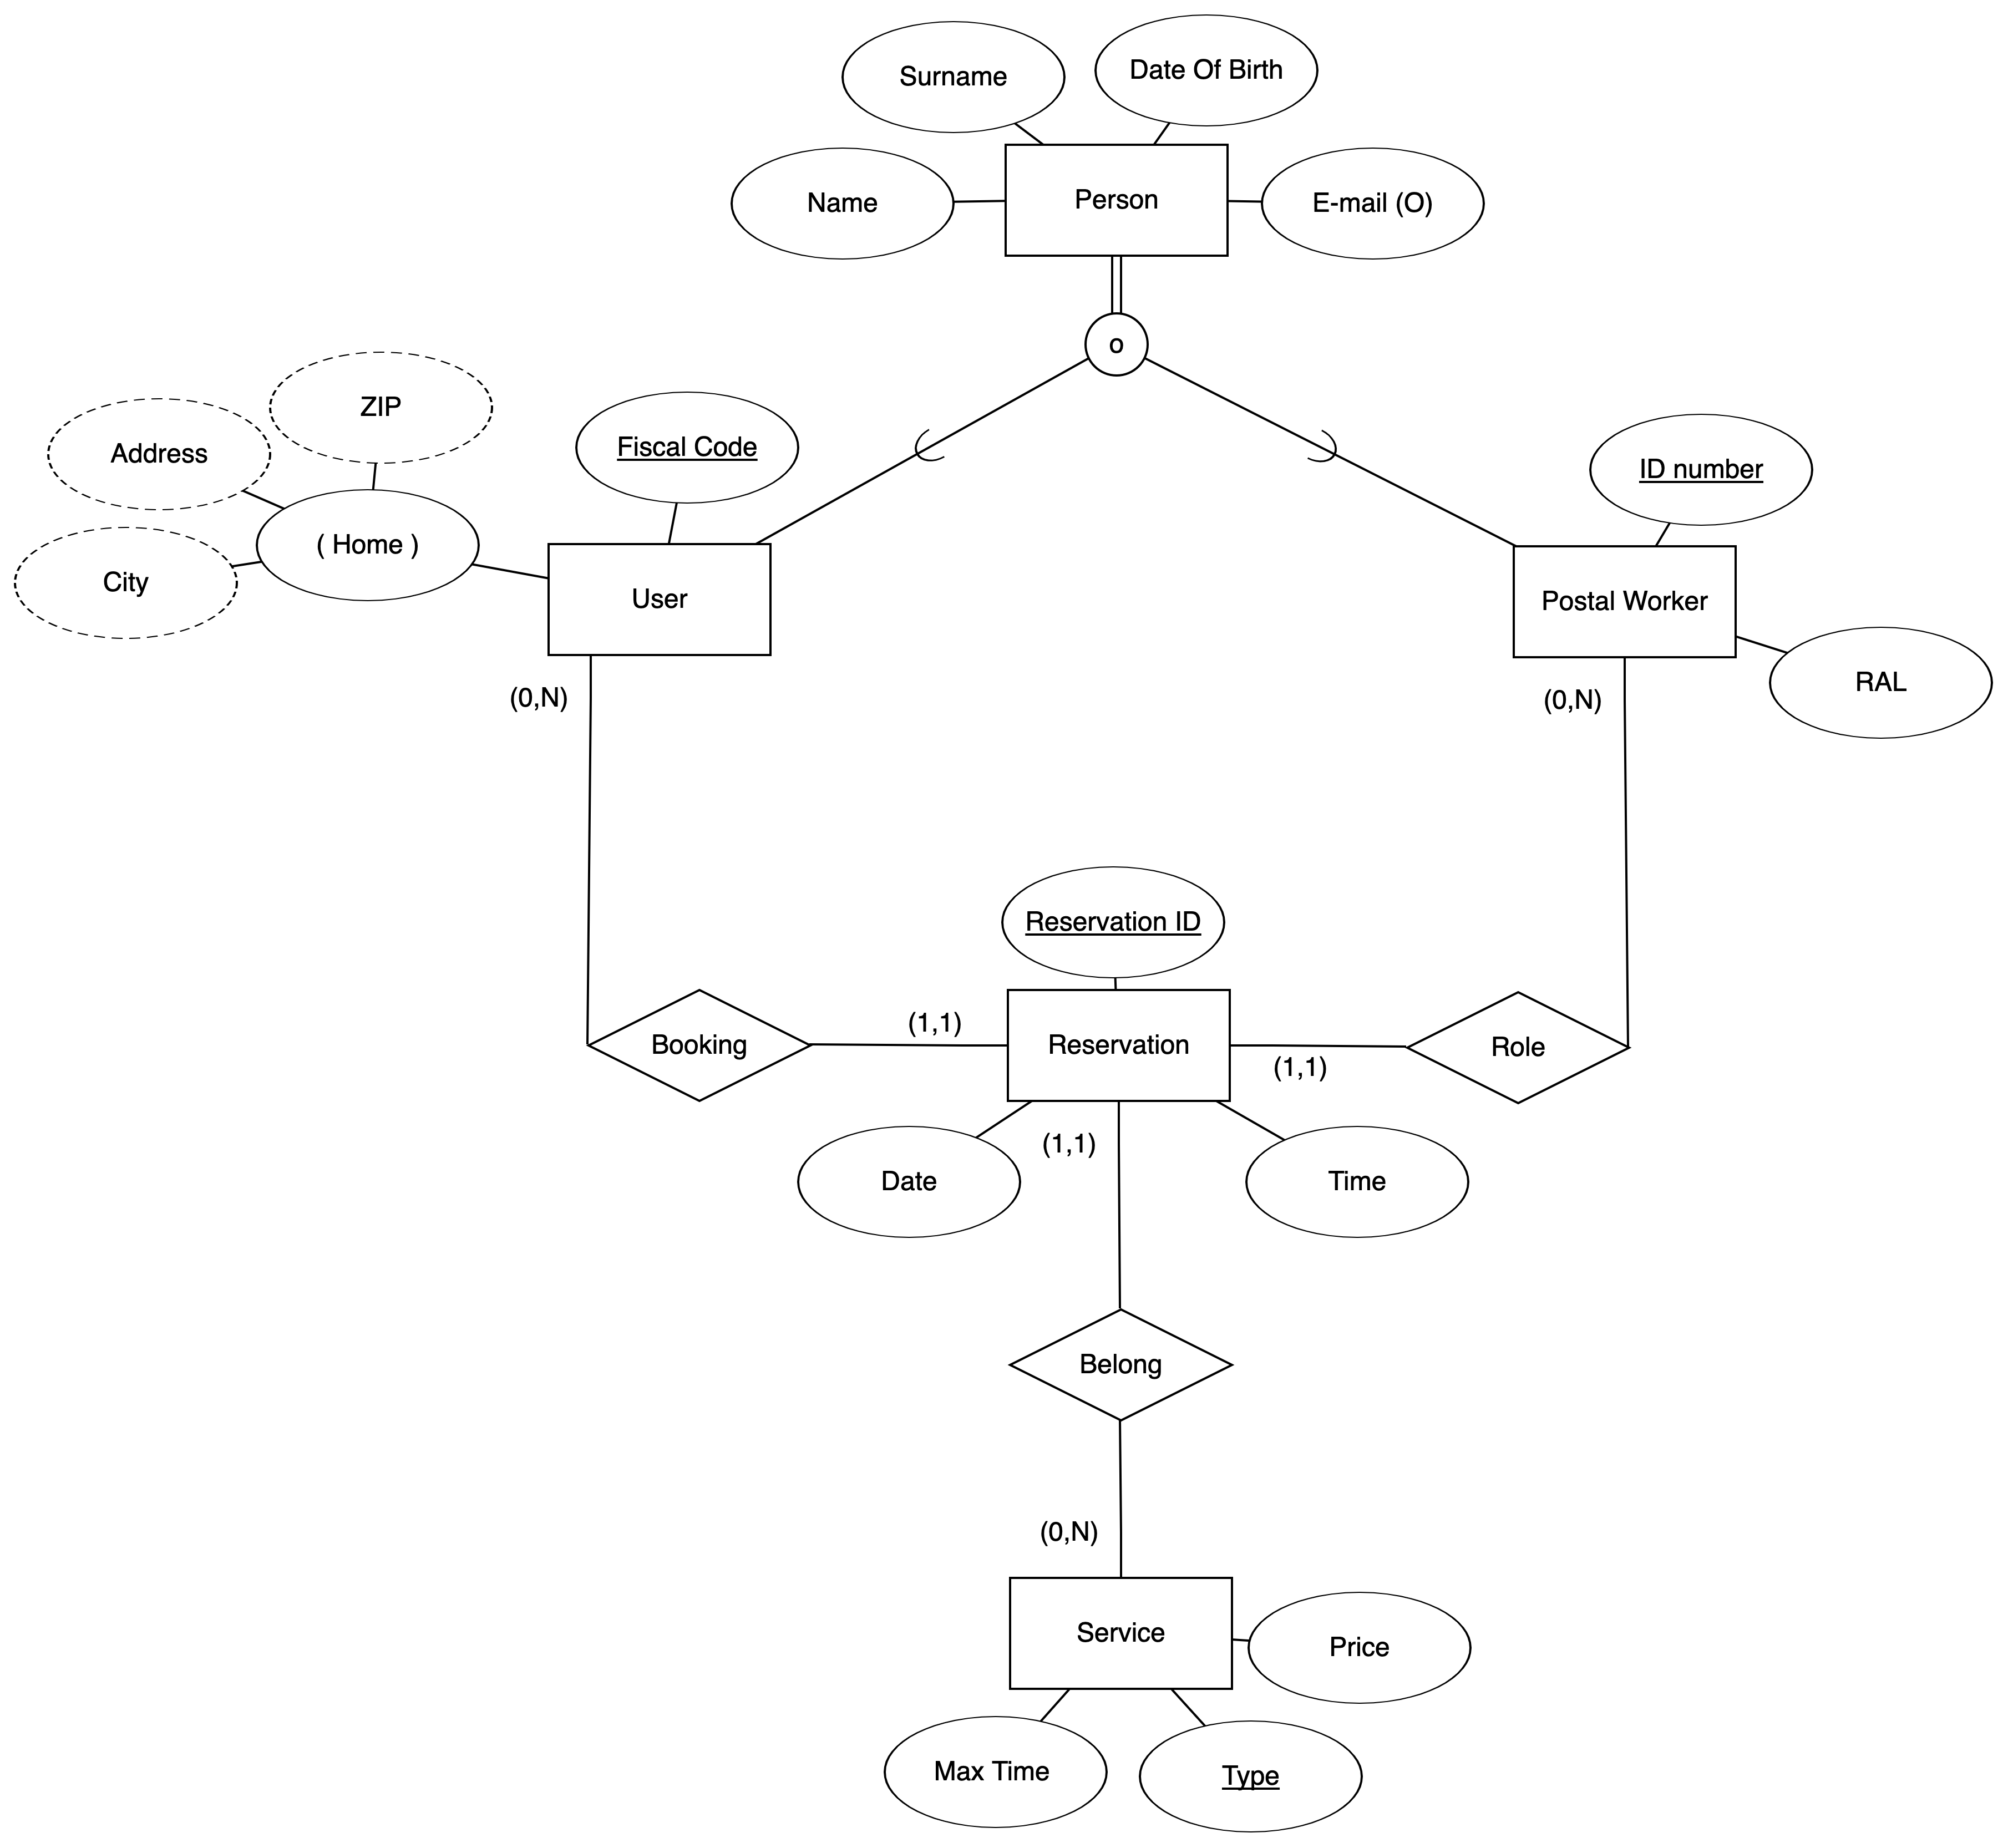
\includegraphics[width=12cm]{images/PostOfficeERdiagram.png}
\end{center}

Notice that we added a generalization relationship between the Users and PostalWorker entities. This is because a postal worker is also a user of the post office services. This generalization relationship allows us to avoid duplicating the information about the postal workers in the Users table. The generalization relationship is total because every postal worker is also a user of the post office services.

Notice that we added a generalization relationship between the Person entity and the User and PostalWorker entities. This is because a user and a postal worker are both people. This generalization relationship allows us to avoid duplicating the information about the people in the Users and PostalWorker tables. The generalization relationship is partial and overlapping because there are person who are not users or postal worker and every postal worker might be a user of the post office.

The relational schema:
\begin{center}
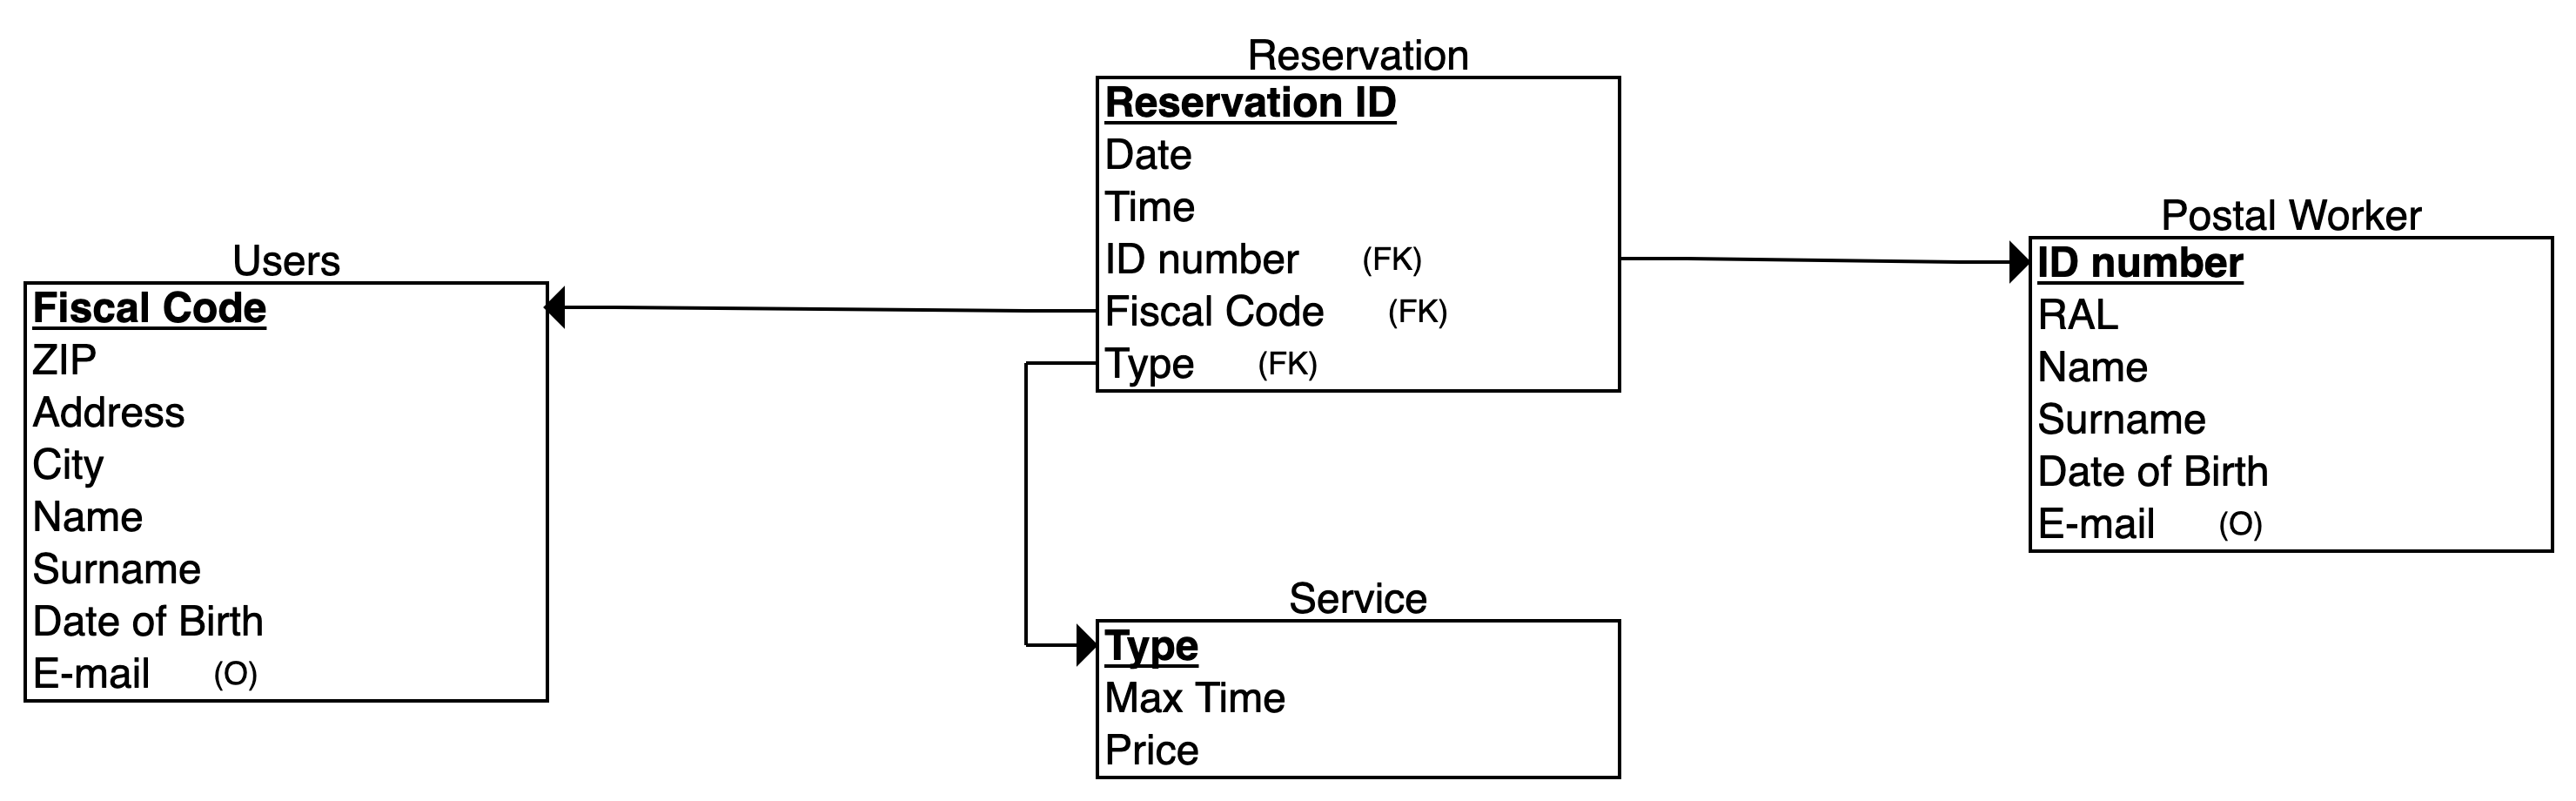
\includegraphics[width=12cm]{images/relationalSchema.png}
\end{center}

\section{Implementation}
% Describe the implementation here
The first step for implementing the database is to create the tables. We used the following SQL code to create the tables:

\begin{lstlisting}[language=SQL]
CREATE TABLE Users (
    FiscalCode char(16) PRIMARY KEY,
    Name varchar(50) NOT NULL,
    Surname varchar(50) NOT NULL,
    DateOfBirth date NOT NULL,
    Email varchar(255),
    City varchar(35) NOT NULL,
    ZIP char(5) NOT NULL,
    Address varchar(100) NOT NULL
);

CREATE TABLE Service (
    Type varchar(255) PRIMARY KEY,
    MaxTime time NOT NULL,
    Price decimal(10,2)
);

CREATE TABLE PostalWorker (
    ID varchar(255) PRIMARY KEY,
    RAL decimal(10,2),
    Name varchar(50) NOT NULL,
    Surname varchar(50) NOT NULL,
    Email varchar(255) UNIQUE
);

CREATE TABLE Reservation (
    ReservationID varchar(255) PRIMARY KEY,
    Date date NOT NULL,
    Time time NOT NULL,
    UserFiscalCode char(16),
    PostalWorkerID varchar(255),
    TypeOfService varchar(255),
    FOREIGN KEY (UserFiscalCode) REFERENCES Users(FiscalCode),
    FOREIGN KEY (PostalWorkerID) REFERENCES PostalWorker(ID),
    FOREIGN KEY (TypeOfService) REFERENCES Service(Type)
);
\end{lstlisting}

Note that the data types are tailored to the data they store. For example, the ZIP code is stored as a string of 5 characters, and the price is stored as a decimal number with 2 decimal places.

These are some constraints we enforced:
\begin{lstlisting}[language=SQL]
    /* ADDING CONSTRAINTS*/
    ALTER TABLE Users ADD CONSTRAINT zip_check CHECK (ZIP ~ '^[0-9]{5}$');
    
    ALTER TABLE Users ADD CONSTRAINT fiscal_code_check CHECK (FiscalCode ~ '^[A-Z]{6}[0-9]{2}[A-Z][0-9]{2}[A-Z][0-9]{3}[A-Z]$');
    
    ALTER TABLE PostalWorker ADD CONSTRAINT email_unique UNIQUE (Email);
    
    ALTER TABLE Service ADD CONSTRAINT price_check CHECK (Price > 0);
    
    ALTER TABLE PostalWorker ADD CONSTRAINT ral_check CHECK (RAL > 0);
\end{lstlisting}

The attributes ZIP and FiscalCode satisfy both the format and the length constraints given. The attributes Price and RAL are greater than 0.

Moreover, we added a trigger to prevent a user from booking two services that overlap in time. Before a new reservation is inserted or an existing reservation is updated, the trigger checks if the user has any other reservations at the same date and time that overlap with the new or updated reservation. If such an overlapping reservation exists, the trigger raises an exception and prevents the operation from completing.
\begin{lstlisting}[language=SQL]
CREATE OR REPLACE FUNCTION check_double_booking() RETURNS TRIGGER AS $$
DECLARE
    overlapping_reservation_count INT;
BEGIN
    SELECT COUNT(*)
    INTO overlapping_reservation_count
    FROM Reservation
    JOIN Service S on S.Type = Reservation.TypeOfService
    WHERE UserFiscalCode = NEW.UserFiscalCode
    AND Date = NEW.Date
      /*  NEGATED New_initial_time > Old_final_time OR New_final_time < old_initial_time

         THERE IS AN OVERLAPPING
            IF the NEW one STARTS BEFORE the OLD one ENDS
         AND
            IF the NEW one ENDS AFTER the OLD one STARTS*/

    AND NEW.Time < (Time + S.MaxTime::interval)
    AND (NEW.Time + (SELECT MaxTime::interval FROM Service WHERE Type = NEW.TypeOfService)) > Time;

    IF overlapping_reservation_count > 0 THEN
        RAISE EXCEPTION 'User cannot book two services at the same time';
    END IF;

    RETURN NEW;
END;
$$ LANGUAGE plpgsql;

CREATE TRIGGER prevent_double_booking
BEFORE INSERT OR UPDATE ON Reservation
FOR EACH ROW EXECUTE PROCEDURE check_double_booking();

\end{lstlisting}
\section{Sample Data}
% Describe the sample data here
Finally, we had to insert some sample data into the database. We will provide some snippets of the SQL code we used to insert the sample data:
\begin{lstlisting}[language=SQL]
INSERT INTO Users (FiscalCode, Name, Surname, DateOfBirth, Email, City, ZIP, Address)
VALUES
('DNSFNC01C24E958W', 'Francesco', 'Doni', '1980-01-01', 'francesco.doni@example.com', 'Rome', '00147', 'Via Roma 10'),

INSERT INTO Service (Type, MaxTime, Price)
VALUES
('Mail', 60, 1.00),
('Bill Payment', 30, 2.00),
('Insurance', 60, 3.00),
('Internet Connectivity', 30, 4.00)

INSERT INTO PostalWorker (ID, RAL, Name, Surname, Email)
VALUES
('PW001', 22000.00, 'Giuseppe', 'Verdi', 'giuseppe.verdi@example.com'),
('PW002', 20500.00, 'Antonio', 'Vivaldi', 'antonio.vivaldi@example.com')

INSERT INTO Reservation (ReservationID, Date, Time, UserFiscalCode, PostalWorkerID, TypeOfService)
VALUES
('R001', '2023-07-15', '09:00:00', 'DNSFNC01C24E958W', 'PW001', 'Bill Payment'),
('R002', '2023-07-15', '09:30:00', 'BLLMRC02D25E958X', 'PW002', 'Internet Connectivity'),
('R003', '2023-07-15', '10:00:00', 'RSSFBA03E26E958Y', 'PW003', 'Insurance'),
('R004', '2023-07-15', '10:30:00', 'VRDLCA04F27E958Z', 'PW004', 'Mail'),
\end{lstlisting}

\section{Sample queries}
% Write some sample queries here
This section was not required. It's just a collection of some sample queries we wrote to test the database.

1. Find all reservations made by a specific user:

\begin{lstlisting}[language=SQL]
SELECT *
FROM Reservation
WHERE UserFiscalCode = 'DNSFNC01C24E958W';
\end{lstlisting}

2. Find the postal worker with the highest RAL\@:

\begin{lstlisting}[language=SQL]
    SELECT * FROM PostalWorker ORDER BY RAL DESC LIMIT 1;
\end{lstlisting}

3. Find the total number of reservations made for each service:

\begin{lstlisting}[language=SQL]
    SELECT Type, COUNT(*)
    FROM Reservation
    GROUP BY Type;
\end{lstlisting}

4. Find all services offered that take less than 30 minutes:

\begin{lstlisting}[language=SQL]
    SELECT *
    FROM Service
    WHERE MaxTime < '00:30:00';
\end{lstlisting}

5. Find all reservations for a specific date:

\begin{lstlisting}[language=SQL]
    SELECT *
    FROM Reservation
    WHERE Date = '2023-07-15';
\end{lstlisting}

6. Find all users who have made a reservation for a specific service

\begin{lstlisting}[language=SQL]
    SELECT Users.* 
    FROM Users 
    JOIN Reservation ON Users.FiscalCode = Reservation.UserFiscalCode 
    WHERE Reservation.TypeOfService = 'Mail';
\end{lstlisting}

\section{Conclusion}
% Write your conclusion here
In conclusion, we manage to create a working database for a post office. We designed the database, implemented it in PostgreSQL, and populated it with sample data. We also wrote some sample queries to test the database. \\
We are almost ready to deploy it!
\end{document}
